% Created 2021-11-13 sáb 20:40
% Intended LaTeX compiler: pdflatex
\documentclass[aspectratio=169, xcolor={usenames,svgnames,dvipsnames}]{beamer}
\usepackage[utf8]{inputenc}
\usepackage[T1]{fontenc}
\usepackage{graphicx}
\usepackage{grffile}
\usepackage{longtable}
\usepackage{wrapfig}
\usepackage{rotating}
\usepackage[normalem]{ulem}
\usepackage{amsmath}
\usepackage{textcomp}
\usepackage{amssymb}
\usepackage{capt-of}
\usepackage{hyperref}
\usepackage{color}
\usepackage{listings}
\usepackage{mathpazo}
\usepackage{gensymb}
\usepackage{amsmath}
\usepackage{diffcoeff}
\usepackage{steinmetz}
\usepackage{mathtools}
\bibliographystyle{plain}
\usepackage{siunitx}
\sisetup{output-decimal-marker=comma}
\DeclareSIUnit{\watthour}{Wh}
\hypersetup{colorlinks=true, linkcolor=Blue, urlcolor=Blue}
\renewcommand{\thefootnote}{\fnsymbol{footnote}}
\newcommand{\laplace}[1]{\mathbf{#1}(\mathbf{s})}
\newcommand{\slp}{\mathbf{s}}
\newcommand{\fasor}[1]{\mathbf{#1}(\omega)}
\newcommand{\atan}{\mathrm{atan}}
\parskip=5pt
\usetheme{Boadilla}
\usecolortheme{rose}
\usefonttheme{serif}
\author{Ana Fernández-Guillamón}
\date{}
\title{Introducción al régimen transitorio}
\setbeamercolor{alerted text}{fg=blue!50!black} \setbeamerfont{alerted text}{series=\bfseries}
\AtBeginSubsection[]{\begin{frame}[plain]\tableofcontents[currentsubsection,sectionstyle=show/shaded,subsectionstyle=show/shaded/hide]\end{frame}}
\AtBeginSection[]{\begin{frame}[plain]\tableofcontents[currentsection,hideallsubsections]\end{frame}}
\beamertemplatenavigationsymbolsempty
\setbeamertemplate{footline}[frame number]
\setbeamertemplate{itemize items}[triangle]
\setbeamertemplate{enumerate items}[circle]
\setbeamertemplate{section in toc}[circle]
\setbeamertemplate{subsection in toc}[circle]
\hypersetup{
 pdfauthor={Oscar Perpiñán Lamigueiro},
 pdftitle={Introducción al régimen transitorio},
 pdfkeywords={},
 pdfsubject={},
 pdfcreator={Emacs 27.1 (Org mode 9.4.6)}, 
 pdflang={Spanish}}
\begin{document}

\maketitle

\section{Formas de onda}


\begin{frame}{Formas de onda}
\begin{itemize}
\item La salida de los generadores (de tensión o de corriente) son funciones que pueden variar con el tiempo
\item La dependencia funcional \(u = u(t)\) o \(i = i(t)\) se denomina \alert{forma de onda}
\item Clasificación:
\begin{itemize}
    \item Signo de la magnitud
    \begin{itemize}
\item Unidireccionales: única polaridad (signo constante), aunque el valor puede ser constante (corriente continua) o variable
\item Bidireccionales: cambio de polaridad (signo variable con el tiempo)
\end{itemize}
\item Repetición del valor de la magnitud:
\begin{itemize}
    \item Periódicas: el valor de la magnitud se repite de forma regular
    \item No periódicas: el valor de la magnitud varía de forma arbitraria con el tiempo
\end{itemize}
\end{itemize}
\end{itemize}
\end{frame}

% \begin{frame}[label={sec:org2c3a4b0}]{Valores que definen una onda periódica}
% \begin{block}{Período y frecuencia}
% \begin{itemize}
% \item Período (\(T\)): tiempo que tarda en repetirse la función.
% \item Frecuencia (\(f\)): número de repeticiones por unidad de tiempo.
% \item \(f = \frac{1}{T}\)
% \end{itemize}
% \end{block}
% \begin{block}{Valor medio}
% \[
% U_m=\frac{1}{T}\int_{0}^{T}u(t)\, dt \qquad \qquad%
% I_m=\frac{1}{T}\int_{0}^{T}i(t)\, dt
% \]
% \end{block}

% \begin{block}{Valor eficaz}
% \[
% U = \sqrt{\frac{1}{T}\cdot\int_{0}^{T}u^{2}(t)\, dt} \qquad \qquad%
% I = \sqrt{\frac{1}{T}\cdot\int_{0}^{T}i^{2}(t)\, dt}
% \]
% \end{block}
% \end{frame}

% \begin{frame}[label={sec:orgf3492e9}]{Valores que definen una onda periódica}
% \begin{itemize}
% \item Valores de pico

% \[
% Y_{max} = \max(y(t)) \qquad Y_{min} = \min(y(t))
% \]

% \item Amplitud o valor pico a pico
% \end{itemize}

% \[
%  |Y_{max} - Y_{min}|
% \]

% \begin{itemize}
% \item Factor de amplitud
% \end{itemize}

% \[FA = \frac{Y_{max}}{Y}\]

% \begin{itemize}
% \item Factor de forma
% \end{itemize}

% \[FF = \frac{Y}{Y_{m}}\]
% \end{frame}

\subsection{Formas de onda básicas}

\begin{frame}{Formas de onda básicas}{Función escalón}
\begin{columns}
\begin{column}{0.5\columnwidth}
\begin{center}
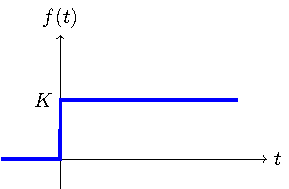
\includegraphics[width=.9\linewidth]{../figs/escalon.pdf}
\end{center}
\end{column}

\begin{column}{0.5\columnwidth}
\[
  f(t) = %
  \begin{cases}
    0 & t < 0\\
    K & t \geq 0
  \end{cases}
  \]
\end{column}
\end{columns}
$K=1\Rightarrow$ escalón unitario
\end{frame}

\begin{frame}{Formas de onda básicas}{Función pulso rectangular}
\begin{columns}
\begin{column}{0.5\columnwidth}
\begin{center}
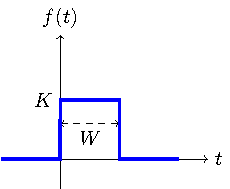
\includegraphics[width=.9\linewidth]{../figs/pulso.pdf}
\end{center}
\end{column}

\begin{column}{0.5\columnwidth}
\[
  f(t) = %
  \begin{cases}
    0 & t < 0\\
    K & 0 \leq t \leq W\\
    0 & t>W
  \end{cases}
  \]
\end{column}
\end{columns}
\end{frame}

\begin{frame}{Formas de onda básicas}{Función rampa}
\begin{columns}
\begin{column}{0.5\columnwidth}
\begin{center}
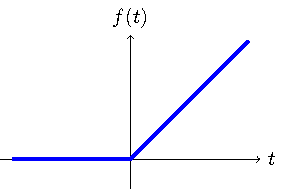
\includegraphics[width=.9\linewidth]{../figs/rampa.pdf}
\end{center}
\end{column}

\begin{column}{0.5\columnwidth}
\[
  f(t) = %
  \begin{cases}
    0 & t < 0\\
    m \cdot t  & t \geq 0
  \end{cases}
  \]
\end{column}
\end{columns}
\end{frame}

\begin{frame}{Formas de onda básicas}{Función triangular}
\begin{columns}
\begin{column}{0.4\columnwidth}
\begin{center}
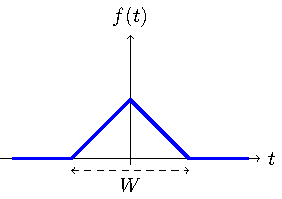
\includegraphics[width=.9\linewidth]{../figs/triangular.pdf}
\end{center}
\end{column}

\begin{column}{0.6\columnwidth}
\[
  f(t) = %
  \begin{cases}
    0 & t < -W/2\\
    m \cdot (t + W/2)  & -W/2 \leq t \leq 0\\
    -m \cdot (t - W/2)  & 0 \leq t \leq W/2\\
    0  & t > W/2
  \end{cases}
  \]
\end{column}
\end{columns}
\end{frame}

\begin{frame}{Formas de onda básicas}{Retraso del origen de tiempos}
Desplazamiento en el eje de ordenadas una cantidad $-t_0$
\begin{columns}
\begin{column}{0.5\linewidth}
\begin{center}
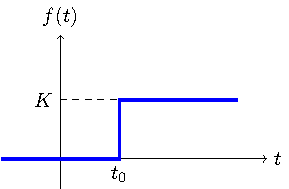
\includegraphics[height=0.35\textheight]{../figs/escalon_t0.pdf}\\
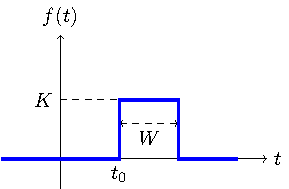
\includegraphics[height=0.35\textheight]{../figs/pulso_t0.pdf}
\end{center}
\end{column}
\begin{column}{0.5\linewidth}
\begin{center}
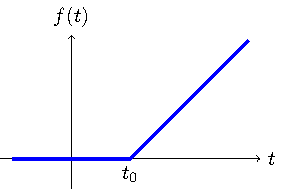
\includegraphics[height=0.35\textheight]{../figs/rampa_t0.pdf}\\
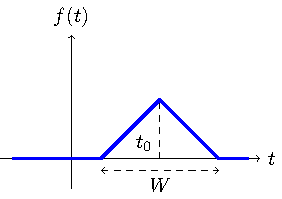
\includegraphics[height=0.35\textheight]{../figs/triangular_t0.pdf}
\end{center}
\end{column}
\end{columns}
\end{frame}

\section{Introducción al régimen transitorio}

\begin{frame}{Introducción al régimen transitorio}
\begin{block}{Régimen transitorio}
\begin{itemize}
\item Cambio en las condiciones de funcionamiento de un circuito: activación o apagado de fuentes, cambio en las cargas, interruptores...
\item Variación de $u(t)$ e $i(t)$ hasta alcanzar nuevos valores $\rightarrow$ circuito estabilizado
\item \alert{Ecuaciones diferenciales}
\end{itemize}
\end{block}
\begin{block}{Régimen permanente o estacionario (circuito estabilizado)}
Las tensiones y corrientes de un circuito son constantes (CC) o periódicas (CA)
\end{block}
\end{frame}

\begin{frame}{Introducción al régimen transitorio}{Ecuaciones diferenciales}
Al aplicar Kirchhoff a un circuito lineal, se obtienen ecuaciones diferenciales: 

\[
  u_L(t) = L \cdot \diff{i_L(t)}{t}
  \leftrightarrow
  i_L(t) = \frac{1}{L} \int^t_{-\infty}u_L(t') \mathrm{d}t'
\]
\[
  i_C(t) = C \cdot \diff{u_C(t)}{t}
  \leftrightarrow
  u_C(t) = \frac{1}{C} \int^t_{-\infty}i_C(t') \mathrm{d}t'
\]

\alert{Importante recordar el operador $D$}
\begin{align*}
	    Z_R(D)&=\dfrac{u_R(t)}{i(t)}=R\\
	    Z_L(D)&=\dfrac{u_L(t)}{i(t)}=LD\\
	    Z_C(D)&=\dfrac{u_C(t)}{i(t)}=\dfrac{1}{CD}
	\end{align*}
\end{frame}

\begin{frame}{Introducción al régimen transitorio}{Respuesta completa de una red lineal}
La solución de esta ecuación diferencial para \(t > 0\) tiene dos componentes:

\[
 \boxed{f(t) = f_n(t) + f_\infty(t) }
 \]

\begin{itemize}
\item Respuesta \alert{natural} o general, \(f_n(t)\):
\begin{itemize}
\item Respuesta sin fuentes
\item Determinada por la energía almacenada previamente y por la configuración del circuito
\item Contiene constantes de integración
\item Resolver \alert{ecuación homogénea}
\end{itemize}
\item Respuesta \alert{forzada} o particular, \(f_\infty(t)\):
\begin{itemize}
\item Determinada por las fuentes existentes en \(t > 0\)
\item Es la respuesta del circuito tras un tiempo suficiente, \(t \to \infty\) (régimen permanente)
\end{itemize}
\end{itemize}
\end{frame}

\section{Condiciones iniciales}

\begin{frame}{Condiciones iniciales}
\begin{itemize}
\item El instante del cambio se representa habitualmente con \(t = 0\):
\begin{itemize}
\item \(t = 0^-\): tiempo inmediatamente anterior al cambio
\item \(t = 0^+\): tiempo inmediatamente posterior al cambio
\end{itemize}

\item Dependen de las \alert{energías almacenadas} en $t=0^-$

\item Se aplican a la \alert{topología} del circuito en \(t = 0^+\)

\item Determinan las constantes de integración
\end{itemize}
\end{frame}

\begin{frame}{Condiciones iniciales}{Resistencia}
No acumula energía: sigue los cambios de forma instantánea.

\[
u(t) = R\cdot i(t)
\]
\end{frame}



\begin{frame}{Condiciones iniciales}{Bobina}
\begin{columns}
\begin{column}{0.5\linewidth}
La corriente no puede variar de forma brusca (implica tensión infinita):
\[
u_L(t) = L \cdot \diff{i_L(t)}{t}
\leftrightarrow
i_L(t) = \frac{1}{L} \int^t_{-\infty}u_L(t') \mathrm{d}t'
\]
\[
\boxed{i_L(0^-) = i_L(0^+)}
\]
\end{column}

\begin{column}{0.5\linewidth}
\begin{center}
    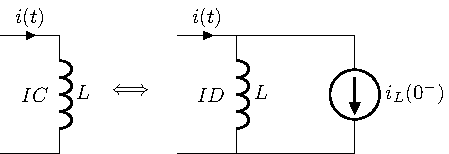
\includegraphics[width=0.8\linewidth]{../figs/condiciones_iniciales_L.pdf}
\end{center}
\end{column}
\end{columns}


\begin{block}{Continuidad en una bobina}
Una bobina inicialmente cargada (IC) se puede sustituir por una fuente ideal de corriente de valor $i_g=i_L(0^+)=i_L(0^-)$ en paralelo con una bobina descargada (ID). Si la bobina está descargada ($i_L(0^-)=0$), se comporta inicialmente como un \alert{circuito abierto}, independientemente de la tensión en sus terminales.
\end{block}
\end{frame}


\begin{frame}{Condiciones iniciales}{Condensador}
\begin{columns}
\begin{column}{0.5\linewidth}
La tensión no puede variar de forma brusca (implica corriente infinita):
\[
i_C(t) = C \cdot \diff{u_C(t)}{t}
\leftrightarrow
u_C(t) = \frac{1}{C} \int^t_{-\infty}i_C(t') \mathrm{d}t'
\]
\[
\boxed{u_C(0^-) = u_C(0^+)}
\]
\end{column}

\begin{column}{0.5\linewidth}
\begin{center}
    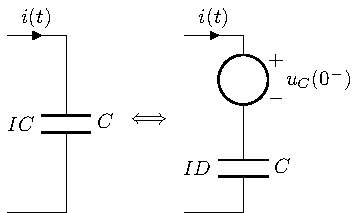
\includegraphics[width=0.8\linewidth]{../figs/condiciones_iniciales_C.pdf}
\end{center}
\end{column}
\end{columns}


\begin{block}{Continuidad en un condensador bobina}
Un condensador inicialmente cargado (IC) se puede sustituir por una fuente ideal de tensión de valor $u_g=u_C(0^+)=u_C(0^-)$ en serie con un condensador descargado (ID). Si el condensador está descargado ($u_C(0^-)=0$), se comporta inicialmente como un \alert{cortocircuito}, independientemente de la corriente que circule por el mismo.
\end{block}
\end{frame}

\begin{frame}{Condiciones iniciales}{Procedimiento general para obtener las condiciones iniciales}

	\begin{enumerate}
		\item Sustituir los generadores de tensión del circuito $\epsilon_g(t)$ por fuentes de tensión continua de valor $\epsilon_g(0^+)$.
		\item Sustituir todos los generadores de corriente del circuito $i_g(t)$ por fuentes de corriente continua de valor $i_g(0^+)$.
		\item Sustituir todas las bobinas cargadas por su circuito equivalente con condiciones iniciales $i_L(0^-)=i_L(0^+)$. Si la corriente inicial en la bobina es 0 ($i_L(0^-)=0$), se sustituye por un circuito abierto.
		\item Sustituir todos los condensadores cargados por su circuito equivalente con condiciones iniciales $u_C(0^+)=u_C(0^-)$. Si la tensión inicial en un condensador es 0 ($u_C(0^-)=0$), se sustituye por un cortocircuito.
		\item En la red resistiva resultante, calcular las corrientes y tensiones iniciales necesarias para el estudio subsiguiente de la red.
	\end{enumerate}
\end{frame}

\begin{frame}{Condiciones iniciales}{Ejemplo}
    \textbf{En la red de la figura, la corriente del generador de intensidad es $i_g(t) = 10\,\mathrm{e}^{-2t}$ A. El interruptor se abre en $t = 0$, siendo los valores iniciales $i_L(0^-) = 0$ A; $u_C(0^-) = -5$ V. Se pide calcular $i_R(0^+)$, $i_C(0^+)$ y $u_L(0^+)$.}
\begin{figure}[H]
    \centering
    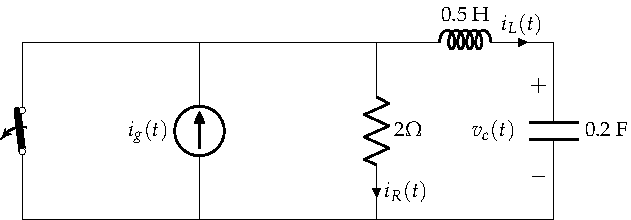
\includegraphics{../figs/ej_condiciones_iniciales.pdf}
\end{figure}
\end{frame}


\section{Circuitos de primer orden}
\begin{frame}{Circuitos de primer orden}{Definición}
\begin{itemize}
\item Circuitos que tienen un \alert{único elemento de acumulación} (o \emph{varios elementos que pueden ser simplificados a un elemento equivalente}) y resistencias
\item \alert{Ecuación diferencial de primer orden}: 
\begin{equation*}
	    a_1\,y'(t)+a_0\,y(t)=g(t)
	\end{equation*}
	\item Resolución:
	\begin{enumerate}
\item Cálculo de las \alert{condiciones iniciales}, analizando el circuito en \(t < 0\)
\item \alert{Respuesta natural}: análisis de la \emph{ecuación homogénea} ($g(t)=0$, sin fuentes) en \(t > 0\):
\begin{equation*}
    y_n(t)=K\,\mathrm{e}^{-\frac{a_0\,t}{a_1}}
\end{equation*}
\item \alert{Respuesta forzada}: análisis del circuito \emph{con fuentes} en \(t > 0\)
\end{enumerate}
\end{itemize}
\end{frame}

\subsection{Circuito RC paralelo}

\begin{frame}{Circuitos de primer orden}{Circuito RC paralelo}
\begin{itemize}
\item En \(t = 0\) se cierra el interruptor
\end{itemize}

\begin{center}
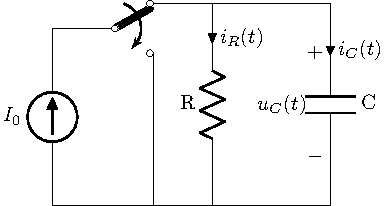
\includegraphics[height=0.45\textheight]{../figs/transitorio_circuitoRC.pdf}
\end{center}
\end{frame}

\begin{frame}{Circuitos de primer orden}{Circuito RC paralelo}
Por 1LK:
\begin{align*}
  \underbrace{i_R(t)}_{\frac{u_C(t)}{R}} + \underbrace{i_C(t)}_{C\,\diff{u_C(t)}{t}} = I_0 \Rightarrow \dfrac{u_C(t)}{R}+C\, u_C'(t)=\dfrac{u_C(t)}{R\,C}+u_C'(t)=\dfrac{I_0}{C}\Rightarrow  \boxed{\dfrac{I_0}{C}=u_C'(t)+\dfrac{1}{R\, C}\,u_C(t)}
\end{align*}
\begin{columns}
\begin{column}{0.6\linewidth}
Respuesta natural: $u_{C,n}(t) = K\,\mathrm{e}^{-\frac{t}{RC}}$

Respuesta forzada: $  u_{C,\infty}(t) = R\cdot I_0$

Respuesta completa:  $u_C(t)=K\,\mathrm{e}^{-\frac{t}{R\,C}}+R\cdot I_0$ 
\begin{itemize}
    \item Usar condiciones iniciales para $K$
\end{itemize}
\end{column}
\begin{column}{0.4\linewidth}
\begin{center}
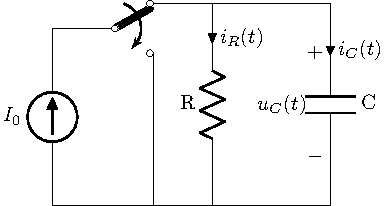
\includegraphics[width=\linewidth]{../figs/transitorio_circuitoRC.pdf}
\end{center}
\end{column}
\end{columns}
\end{frame}

\begin{frame}{Circuitos de primer orden}{Circuito RC paralelo --- Constante de tiempo}
\begin{columns}
\begin{column}{0.5\linewidth}
\begin{itemize}
\item \(\tau = R\cdot C\) [s]
\item Tiempo necesario para que el condensador se cargue al 63\% $(1-1/\mathrm{e})$ de su capacidad
\item $C$ completamente cargado si $t>5\tau$
\item \href{https://www.herramientasingenieria.com/onlinecalc/spa/carga-condensadores/carga-condensadores.html}{Enlace}
\end{itemize}
\end{column}
\begin{column}{0.5\linewidth}
\begin{center}
    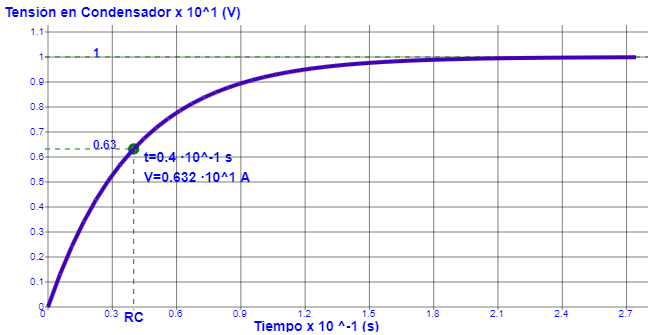
\includegraphics[width=\linewidth]{../figs/tau_RC.PNG}
\end{center}
\end{column}
\end{columns}

\end{frame}


\begin{frame}{Circuitos de primer orden}{Circuito RC paralelo --- Expresión general de la respuesta completa}
\[
\boxed{u_C(t) = \left[u_C(0^+) - u_{C,\infty}(0^+)\right] \mathrm{e}^{-t/\tau} + u_{C,\infty(t)}}
\]

\begin{itemize}
\item \(u_C(0^+)\): tensión en el condensador, condiciones iniciales, \(u(0^-) = u(0^+)\)
\item \(u_{C,\infty(t)}\): tensión en el condensador en régimen permanente para \(t > 0\)
\item \(u_{C,\infty(0^+)}\): tensión en el condensador en régimen permanente particularizada en \(t = 0\)
\end{itemize}
\end{frame}

\subsection{Circuito RL serie}

\begin{frame}{Circuitos de primer orden}{Circuito RL serie}
\begin{itemize}
\item En \(t = 0\) se cierra el interruptor $\Rightarrow i_R(t)=i_L(t)$
\end{itemize}
\begin{center}
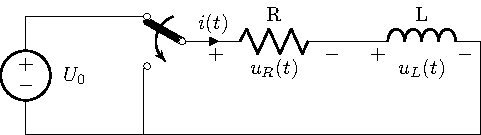
\includegraphics{../figs/transitorio_circuitoRL.pdf}
\end{center}
\end{frame}

\begin{frame}{Circuitos de primer orden}{Circuito RL serie}
Por 2LK:
\begin{align*}
  \underbrace{u_R(t)}_{R\,i_L(t)} + \underbrace{u_L(t)}_{L\,\diff{i_L(t)}{t}} = U_0 \Rightarrow R\,i_L(t)+L\, i_L'(t)=\dfrac{R}{L}\,i_L+i_L'(t)=\dfrac{U_0}{L}\Rightarrow \boxed{\dfrac{U_0}{L}=i_L'(t)+\dfrac{R}{L}\,i_L(t)}
\end{align*}
\begin{columns}
\begin{column}{0.6\linewidth}
Respuesta natural: $i_{L,n}(t) = K\,\mathrm{e}^{-\frac{R\,t}{L}} $

Respuesta forzada: $  i_{L,\infty}(t) = \dfrac{U_0}{R}$ 

Respuesta completa: $i_L(t)=K\,\mathrm{e}^{-\frac{R\,t}{L}}+\dfrac{U_0}{R}$
\begin{itemize}
    \item Usar condiciones iniciales para $K$
\end{itemize}
\end{column}
\begin{column}{0.4\linewidth}
\begin{center}
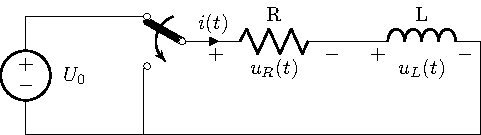
\includegraphics[width=\linewidth]{../figs/transitorio_circuitoRL.pdf}
\end{center}
\end{column}
\end{columns}
\end{frame}

\begin{frame}{Circuitos de primer orden}{Circuito RL serie --- Constante de tiempo}
\begin{itemize}
\item \(\tau = \dfrac{L}{R}\) [s]
\item Tiempo necesario para que por la bobina circule el 63\% de la máxima corriente
\item $L$ a máxima corriente si $t>5\tau$
\item \href{https://es.khanacademy.org/science/electrical-engineering/ee-circuit-analysis-topic/ee-natural-and-forced-response/a/ee-rl-natural-response}{Enlace}
\end{itemize}
\begin{center}
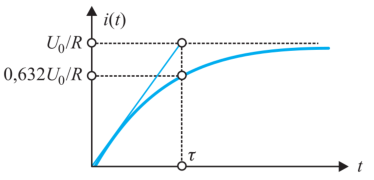
\includegraphics[height=0.45\textheight]{../figs/RespuestaCompleta_RL.pdf}
\end{center}
\end{frame}


\begin{frame}{Circuitos de primer orden}{Circuito RL serie --- Expresión general de la respuesta completa}
\[
\boxed{i_L(t) = \left[i_L(0^+) - i_{L,\infty}(0^+)\right] \mathrm{e}^{-t/\tau} + i_{L,\infty(t)}}
\]

\begin{itemize}
\item \(i_L(0^+)\): corriente en la bobina, condiciones iniciales, \(i_L(0^-) = i_L(0^+)\)
\item \(i_{L,\infty}(t)\): corriente en la bobina en régimen permanente para \(t > 0\)
\item \(i_{L,\infty}(0^+)\): corriente en la bobina en régimen permanente particularizada en \(t = 0\)
\end{itemize}
\end{frame}

\subsection{Procedimiento general}

\begin{frame}{Procedimiento general}
\begin{columns}
\begin{column}{0.6\linewidth}
\begin{center}
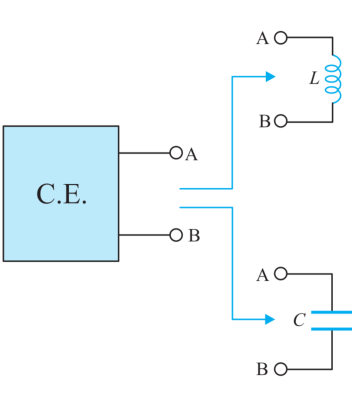
\includegraphics[width=0.6\linewidth]{../figs/CE_primerorden.pdf}
\end{center}
\end{column}
\begin{column}{0.4\linewidth}
\begin{center}
	    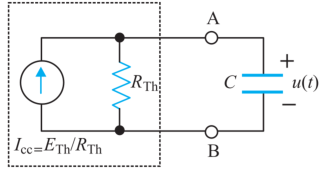
\includegraphics[width=0.8\linewidth]{../figs/thevenin_1orden_C.pdf}\\
	    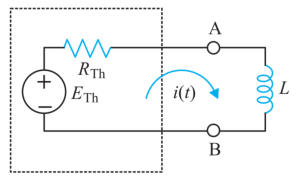
\includegraphics[width=0.8\linewidth]{../figs/thevenin_1orden_L.pdf}
	\end{center}
\end{column}
\end{columns}
\alert{$R_{th}$ es la resistencia vista desde los bornes del condensador o de la bobina, cuando se anulan todas las fuentes independientes}
\end{frame}

\begin{frame}{Procedimiento general}
\begin{enumerate}
\item Dibujar el circuito para $t < 0$:
        \begin{itemize}
        \item Obtener el valor de $i_L(0^-)$ o $u_C(0^-)$
        \item Aplicar el principio de continuidad para determinar $i_L(0^+)$ o $u_C(0^+)$ 
        \end{itemize}
    \item Dibujar el circuito para \(t > 0\):
        \begin{itemize}
        \item Calcular el equivalente de Thévenin/Norton visto por el condensador/bobina
        \item Determinar la constante de tiempo del circuito:
        \begin{equation*}
            \tau = \dfrac{L}{R_{th}} \qquad\qquad \tau = R_{th}\,{C}
        \end{equation*}
        \item Calcular la respuesta en régimen permanente ($i_\infty(t)$ o $u_\infty(t)$):
        \begin{enumerate}
	        \item \textit{Corriente continua}: sustituir la bobina por un cortocircuito y el condensador por un circuito abierto
	        \item \textit{Corriente alterna senoidal}: resolver el circuito por el método fasorial
	        \item \textit{Otro tipo de forma de onda}: determinar la solución particular de la ecuación diferencial
	    \end{enumerate}
        \end{itemize}
    \item Escribir la solución completa para $t>0$:
    \begin{align*}
    i_L(t) &= \left(i_L(0^+) - i_\infty(0^+)\right) e^{-\frac{t}{\tau}} + i_\infty(t)\\
    u_C(t) &= \left(u_C(0^+) - u_\infty(0^+)\right) e^{-\frac{t}{\tau}} + u_\infty(t)\\
    \end{align*}
	\end{enumerate}
\end{frame}

\begin{frame}{Circuitos de primer orden}{Ejemplo 1}
    \textbf{En el circuito de la figura, calcular la corriente $i(t)$ al cerrar el interruptor en $t = 0$ s.}
	    \begin{figure}[H]
	        \centering
	        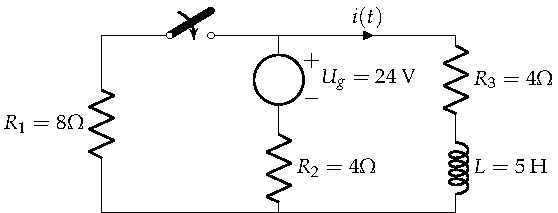
\includegraphics{../figs/ej_transitorio_1orden.pdf}
	    \end{figure}
\end{frame}

\begin{frame}{Circuitos de primer orden}{Ejemplo 2}
    \textbf{El conmutador del circuito de la figura pasa de la posición a 1 a la 2 en $t = 0$ s. Calcular la tensión en bornes de la bobina $t > 0$ s.}
	
	\begin{figure}[H]
	    \centering
	    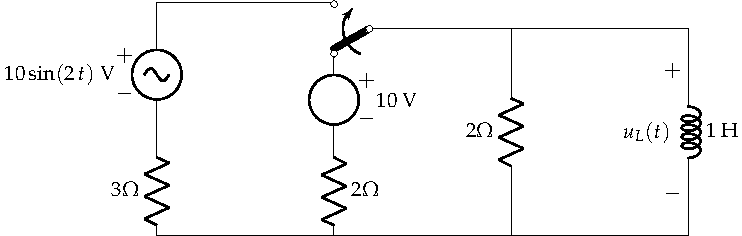
\includegraphics{../figs/ej_transitorio_1orden_AC.pdf}
	\end{figure}
\end{frame}


\section{Circuitos de segundo orden}

\begin{frame}{Circuitos de segundo orden}
\begin{itemize}
\item Circuitos que tienen \alert{dos elementos de acumulación} (o más no asociados en serie/paralelo)
\item \alert{Ecuación diferencial de segundo orden}: 
\begin{equation*}
	    a_2\,y''(t)+a_1\,y'(t)+a_0\,y(t)=g(t)
	\end{equation*}
	\item El método de resolución analiza el circuito en dos etapas:
\begin{itemize}
\item \alert{Respuesta natural} (ecuación diferencial homogénea, sin fuentes) 
\item \alert{Respuesta forzada} (ecuación completa, con fuentes)
\end{itemize}
\end{itemize}
\end{frame}

\subsection{Solución natural}

\begin{frame}{Circuitos de segundo orden}{Solución natural}
    
	\begin{equation*}
	    a_2\,y''(t)+a_1\,y'(t)+a_0\,y(t)=0\Rightarrow \boxed{y''(t)+\dfrac{a_1}{a_2}\,y'(t)+\dfrac{a_0}{a_2}y(t)=0}
	\end{equation*}
	\begin{itemize}
	    \item Cambios de variable:
	    \begin{equation*}
	    {\dfrac{a_1}{a_0}=2\,\xi\,\omega_n}\qquad \qquad {\dfrac{a_0}{a_2}=\omega_n^2}
	\end{equation*}
	\begin{description}
	\item [$\omega_n$] pulsación natural no amortiguada
	\item [$\xi$] coeficiente de amortiguamiento
	\end{description}
	\item Resolver el polinomio característico:
	\begin{equation*}
	    \lambda^2+2\,\xi\,\omega_n\,\lambda + \omega_n^2=0\Rightarrow
	    \begin{cases}
	      \lambda_1=-\omega_n\left(\xi+\sqrt{\xi^2-1} \right)\\ \lambda_2=-\omega_n\left(\xi-\sqrt{\xi^2-1} \right)
	    \end{cases}
	\end{equation*}
	\end{itemize}
\end{frame}

\begin{frame}{Circuitos de segundo orden}{Solución natural}
\begin{columns}
\begin{column}{0.5\linewidth}
\begin{center}
  \alert{Sistema sobreamortiguado ($\xi>1$)}
  \begin{itemize}
      \item $\lambda_1\neq\lambda_2$
      \item Respuesta natural:
      \begin{equation*}
	 y_g(t)=K_1\,\mathrm{e}^{\lambda_1\,t}+K_2\,\mathrm{e}^{\lambda_2\,t}   
	\end{equation*}
  \end{itemize}

\alert{Sistema críticamente amortiguado ($\xi=1$)}  
\begin{itemize}
    \item $\lambda_1=\lambda_2=-\xi\,\omega_n=-\omega_n$
    \item Respuesta natural: 
    \begin{equation*}
	 y_g(t)=\mathrm{e}^{-\omega_n\,t}(K_1\,+K_2\,t)   
	\end{equation*}
\end{itemize}
\end{center}
\end{column}
\begin{column}{0.5\linewidth}
\begin{center}
    \alert{Sistema subamortiguado ($0<\xi<1$)}
\begin{itemize}
    \item $\lambda=a\pm b\,\mathrm{i}=-\omega_n\,\xi\pm \omega_n\,\sqrt{1-\xi^2}\,\mathrm{i}$
    \item Respuesta natural: 
    \begin{align*}
	 &y_g(t)=\mathrm{e}^{-\omega_n\,\xi \,t}[K_1\,\cos(\omega_n\,\sqrt{1-\xi^2}\,t)+\\
	 &+K_2\,\sin(\omega_n\,\sqrt{1-\xi^2}\,t)]  
	\end{align*}
	que puede escribirse como: 
	\begin{equation*}
	 y_g(t)=M\,\mathrm{e}^{-\omega_n\,\xi \,t}\,\sin\left(\omega_n\,\sqrt{1-\xi^2}\,t + \theta \right)
	\end{equation*}
	donde $M=\sqrt{K_1^2+K_2^2}$ y $\tan(\theta)=\frac{K_2}{K_1}$
\end{itemize}
% \alert{Sistema no amortiguado ($\xi=0$)}
% \begin{itemize}
%     \item $\lambda=\pm \omega_n\,\mathrm{i}$
%     \item Respuesta natural: 
%     \begin{equation*}
% 	 y_g(t)=M\,\sin\left(\omega_n\,t + \theta \right)
% 	\end{equation*}
	
% \end{itemize}
\end{center}
\end{column}
\end{columns}
\end{frame}

\subsection{Solución forzada}
\begin{frame}{Circuitos de segundo orden}{Solución forzada}
    $y_\infty(t)$, depende del tipo de alimentación del circuito:
	\begin{itemize}
	        \item \textit{Corriente continua}: sustituir las bobinas por cortocircuitos y los condensadores por circuitos abiertos
	        \item \textit{Corriente alterna senoidal}: resolver el circuito por el método fasorial
	        \item \textit{Otro tipo de forma de onda}: determinar la solución particular de la ecuación diferencial
	    \end{itemize}
\end{frame}

\subsection{Constantes de integración}

\begin{frame}{Circuitos de segundo orden}{Constantes de integración}
    \begin{enumerate}
	    \item Dibujar el circuito en el instante $t=0^+$, sustituyendo las bobinas y condensadores por fuentes de intensidad y tensión, respectivamente, de valor $i_L(0^+)$ y $u_C(0^+)$
	    \item Con este nuevo circuito, puramente resistivo, cualquier variable se puede obtener por superposición $\rightarrow$ se obtiene la primera condición de contorno
	    \item Derivar la expresión de la variable en estudio, particularizada para $t=0^+$ $\rightarrow$ se obtiene la segunda condición de contorno
	    \item Resolver el sistema de 2 ecuaciones con 2 incógnitas
	\end{enumerate}
\end{frame}

\subsection{Procedimiento general}
\begin{frame}{Circuitos de segundo orden}{Procedimiento general}
    \begin{enumerate}
	\item Dibujar el circuito para $t < 0$:
        \begin{itemize}
        \item Obtener los valores de $i_L(0^-)$ y $u_C(0^-)$
        \item Aplicar el principio de continuidad para determinar $i_L(0^+)$ y $u_C(0^+)$
        \end{itemize}
    \item Dibujar el circuito para \(t > 0\), caracterizando los elementos pasivos por su impedancia operacional:
        \begin{itemize}
        \item Obtener la ecuación diferencial del sistema aplicando métodos de análisis generales 
        \item Determinar la solución natural de la ecuación diferencial, especificando también el tipo de sistema 
        \item Calcular la respuesta forzada, según el tipo de alimentación del circuito
        \end{itemize}
        \item Determinar las constantes de la ecuación 
    \item Escribir la solución completa para $t>0$
    \end{enumerate}
\end{frame}

\begin{frame}{Circuitos de segundo orden}{Ejemplo}
    \textbf{El circuito de la figura lleva en la situación indicada un tiempo suficientemente grande, de forma que se encuentra en régimen permanente. En el instante $t=0$, se cierra el interruptor. Determinar la intensidad $i(t)$ para $t>0$. }
	    \begin{figure}[H]
	        \centering
	        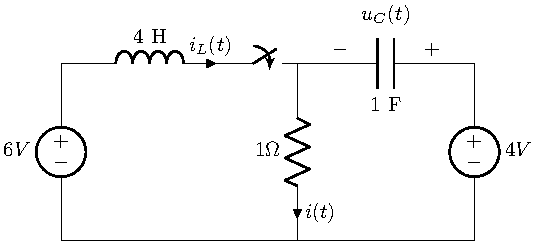
\includegraphics{../figs/ejemplo_2orden.pdf}
	    \end{figure}
\end{frame}

\end{document}